
\chapter{METHODOLOGY}
{\baselineskip=2\baselineskip

This chapter details the design and development of the automated eggplant sorting and grading system, following the Modified Waterfall SDLC model. Section 3.1 discusses the research design and procedural framework. Section 3.2 focuses on the hardware development, describing the design, architecture, and components essential of the conveyor and sorting mechanism. Section 3.3 explains the software development process, detailing the algorithms, tools, and models used for image processing, feature extraction, and classification. Section 3.4 elaborates on the system integration, illustrating how the hardware and software components interact to achieve seamless automation. Collectively, this chapter provides a comprehensive overview of the methods used to ensure the system's accuracy and reliability.

\section{Research Design and Procedure}
This study adopts the Modified Waterfall System Development Life Cycle (SDLC) model as the primary framework for the systematic development of the project. The Modified Waterfall model follows a structured and sequential design process, allowing limited feedback between phases when necessary. This approach ensures that each stage is properly analyzed and refined before proceeding to the next, promoting accuracy, consistency, and efficiency throughout system development. The research design of the study follows these distinct phases, as represented in Figure \ref{fig:researchdesign}.

\begin{figure}
	\centering
	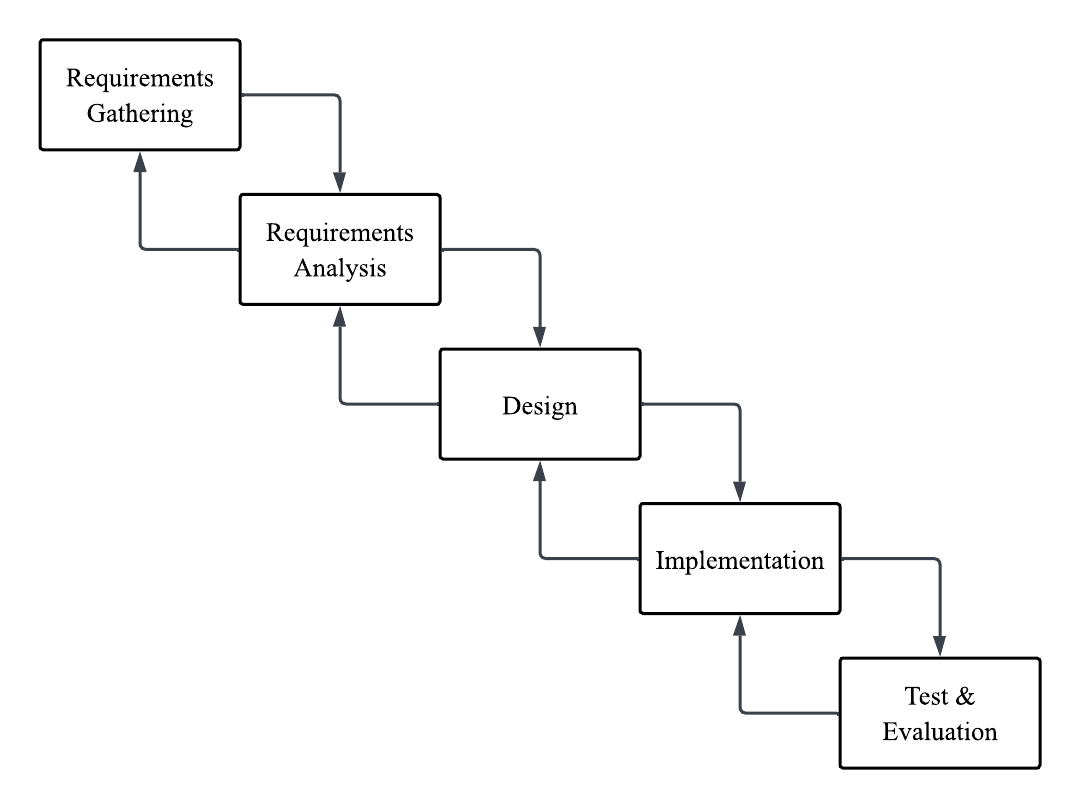
\includegraphics[width=0.7\linewidth]{figures/research_design}
	\caption{Modified Waterfall Model of SDLC}
	\label{fig:researchdesign}
\end{figure}

The development will begin with requirements gathering, where the researchers will collect relevant information from local farmers and agricultural experts to determine the necessity and specifications for automating eggplant sorting and disease detection.  This will be followed by requirements analysis, where the system’s functional requirements and non-functional requirements will be formally defined.

During the design phase, the overall system architecture will be planned. This includes the hardware setup, featuring camera modules for image capture and conveyors with actuators for sorting. The software framework will also be designed to manage image processing, feature extraction, and machine learning-based classification for grading.

In the implementation phase, the designed hardware and software components will be developed and integrated. The program will be coded and linked to the physical components such as cameras, motors, actuators, and controllers to perform automated grading and sorting. Finally, the testing and evaluation phase will assess the prototype's grading accuracy. The results will be analyzed to identify errors or limitations, guiding refinements to improve the system’s accuracy, and reliability.

\section{Hardware Development}
This section presents the design and integration of the system’s mechanical and electronic components. The hardware consists of a conveyor system, camera modules, actuators, and a microcontroller that operate together to transport, classify, and sort eggplants. Each component is configured to function in coordination with the software, ensuring synchronized operation and accurate sorting based on the detected quality of the eggplant. 

\subsection{Hardware Requirements}
The hardware requirements include all the physical components essential for constructing the system. Each component is selected based on its purpose and function in the automated eggplant grading and sorting system, ensuring effective integration and reliable operation to achieve accurate grading and sorting performance.

\begin{longtable}{
		>{\centering\arraybackslash}m{3cm}  
		>{\centering\arraybackslash}m{4cm} 
		>{\arraybackslash}m{6cm}
	}
	\caption{Hardware Requirements} \label{tab:hardwarerequirements} \\
	\toprule
	\multicolumn{1}{c}{\textbf{Component}} &
	\multicolumn{1}{c}{\textbf{Image}} &
	\multicolumn{1}{c}{\textbf{Function}} \\
	\midrule
	
	\endfirsthead
	
	\midrule
	\endhead
	
	\bottomrule
	\endfoot
	
	DC Motor & 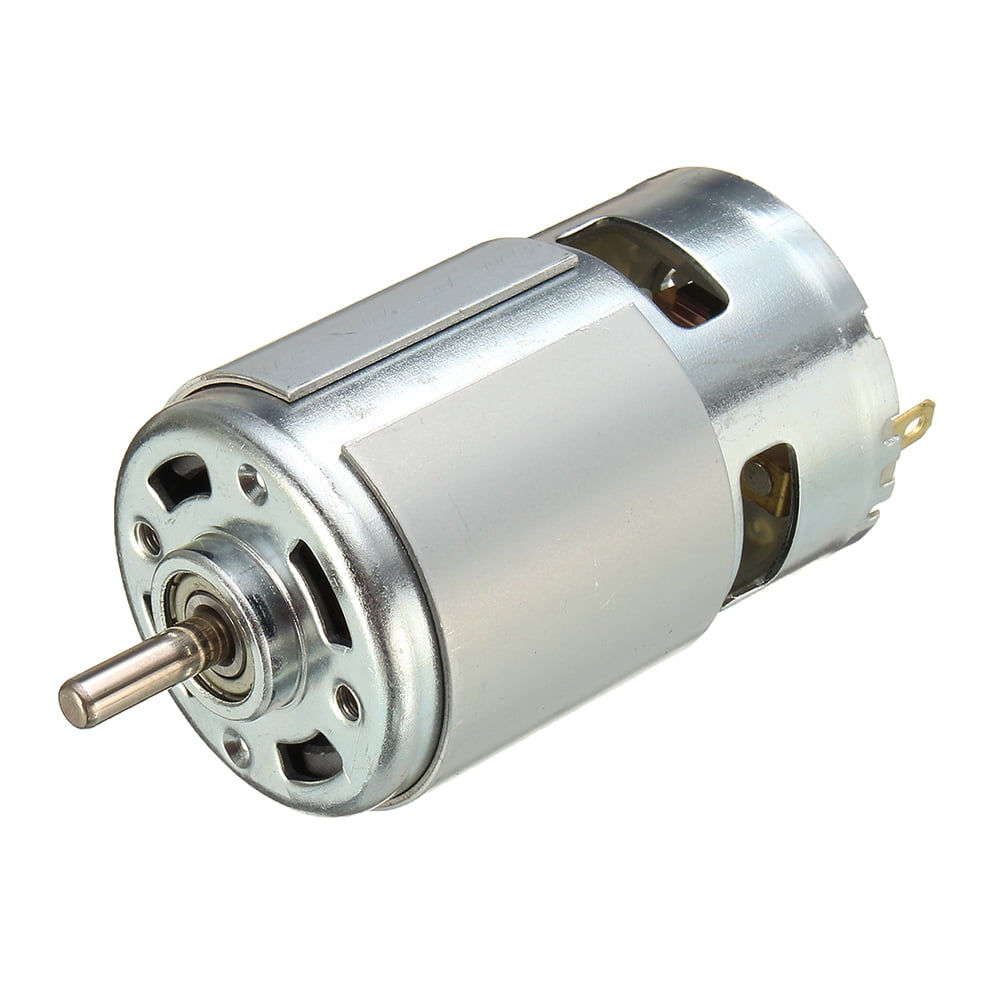
\includegraphics[width=3cm]{figures/dc_motor} &
	This component powers the conveyor belt by converting electrical energy into mechanical motion. \\
	
	Power Supply Adapter & 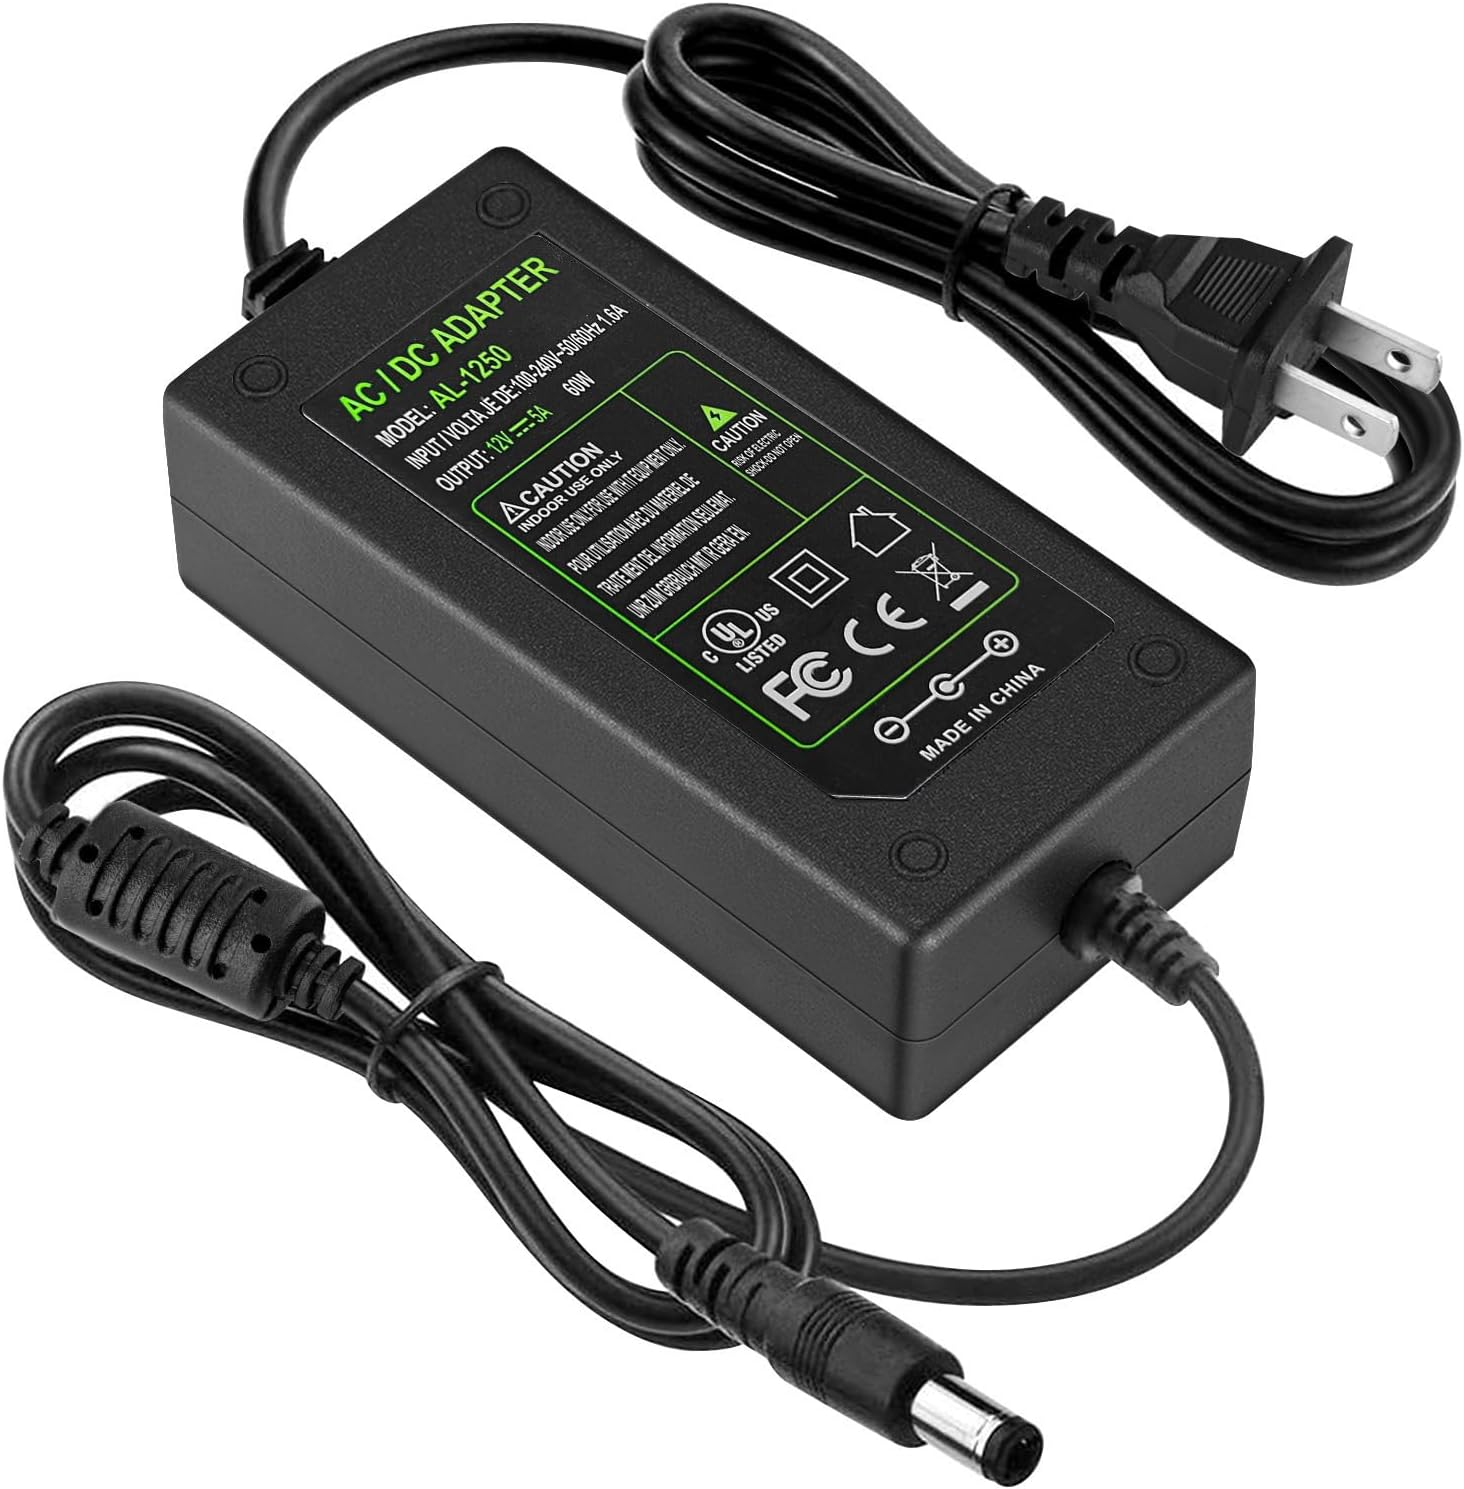
\includegraphics[width=3cm]{figures/adapter} &
	This component supplies the necessary electrical power for the Arduino to operate effectively. \\
	
	Arduino & 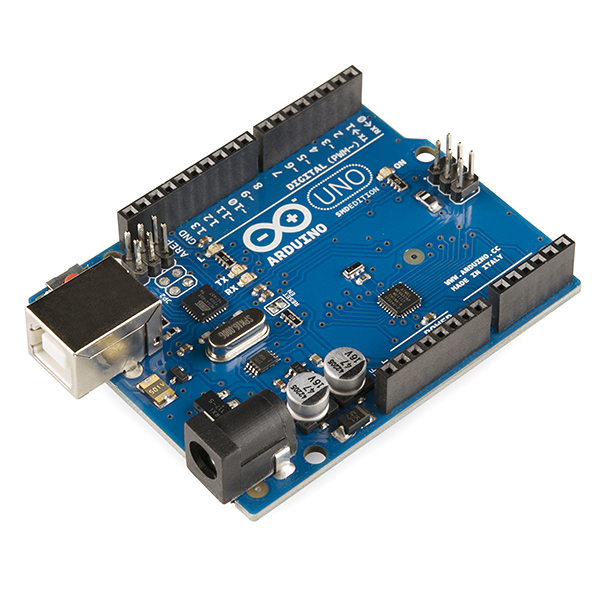
\includegraphics[width=3cm]{figures/arduino} &
	Functions as the control unit for the conveyor belt and actuators, managing the movement and sorting operations of the system based on the classification results. \\
	
	Buck Converter & 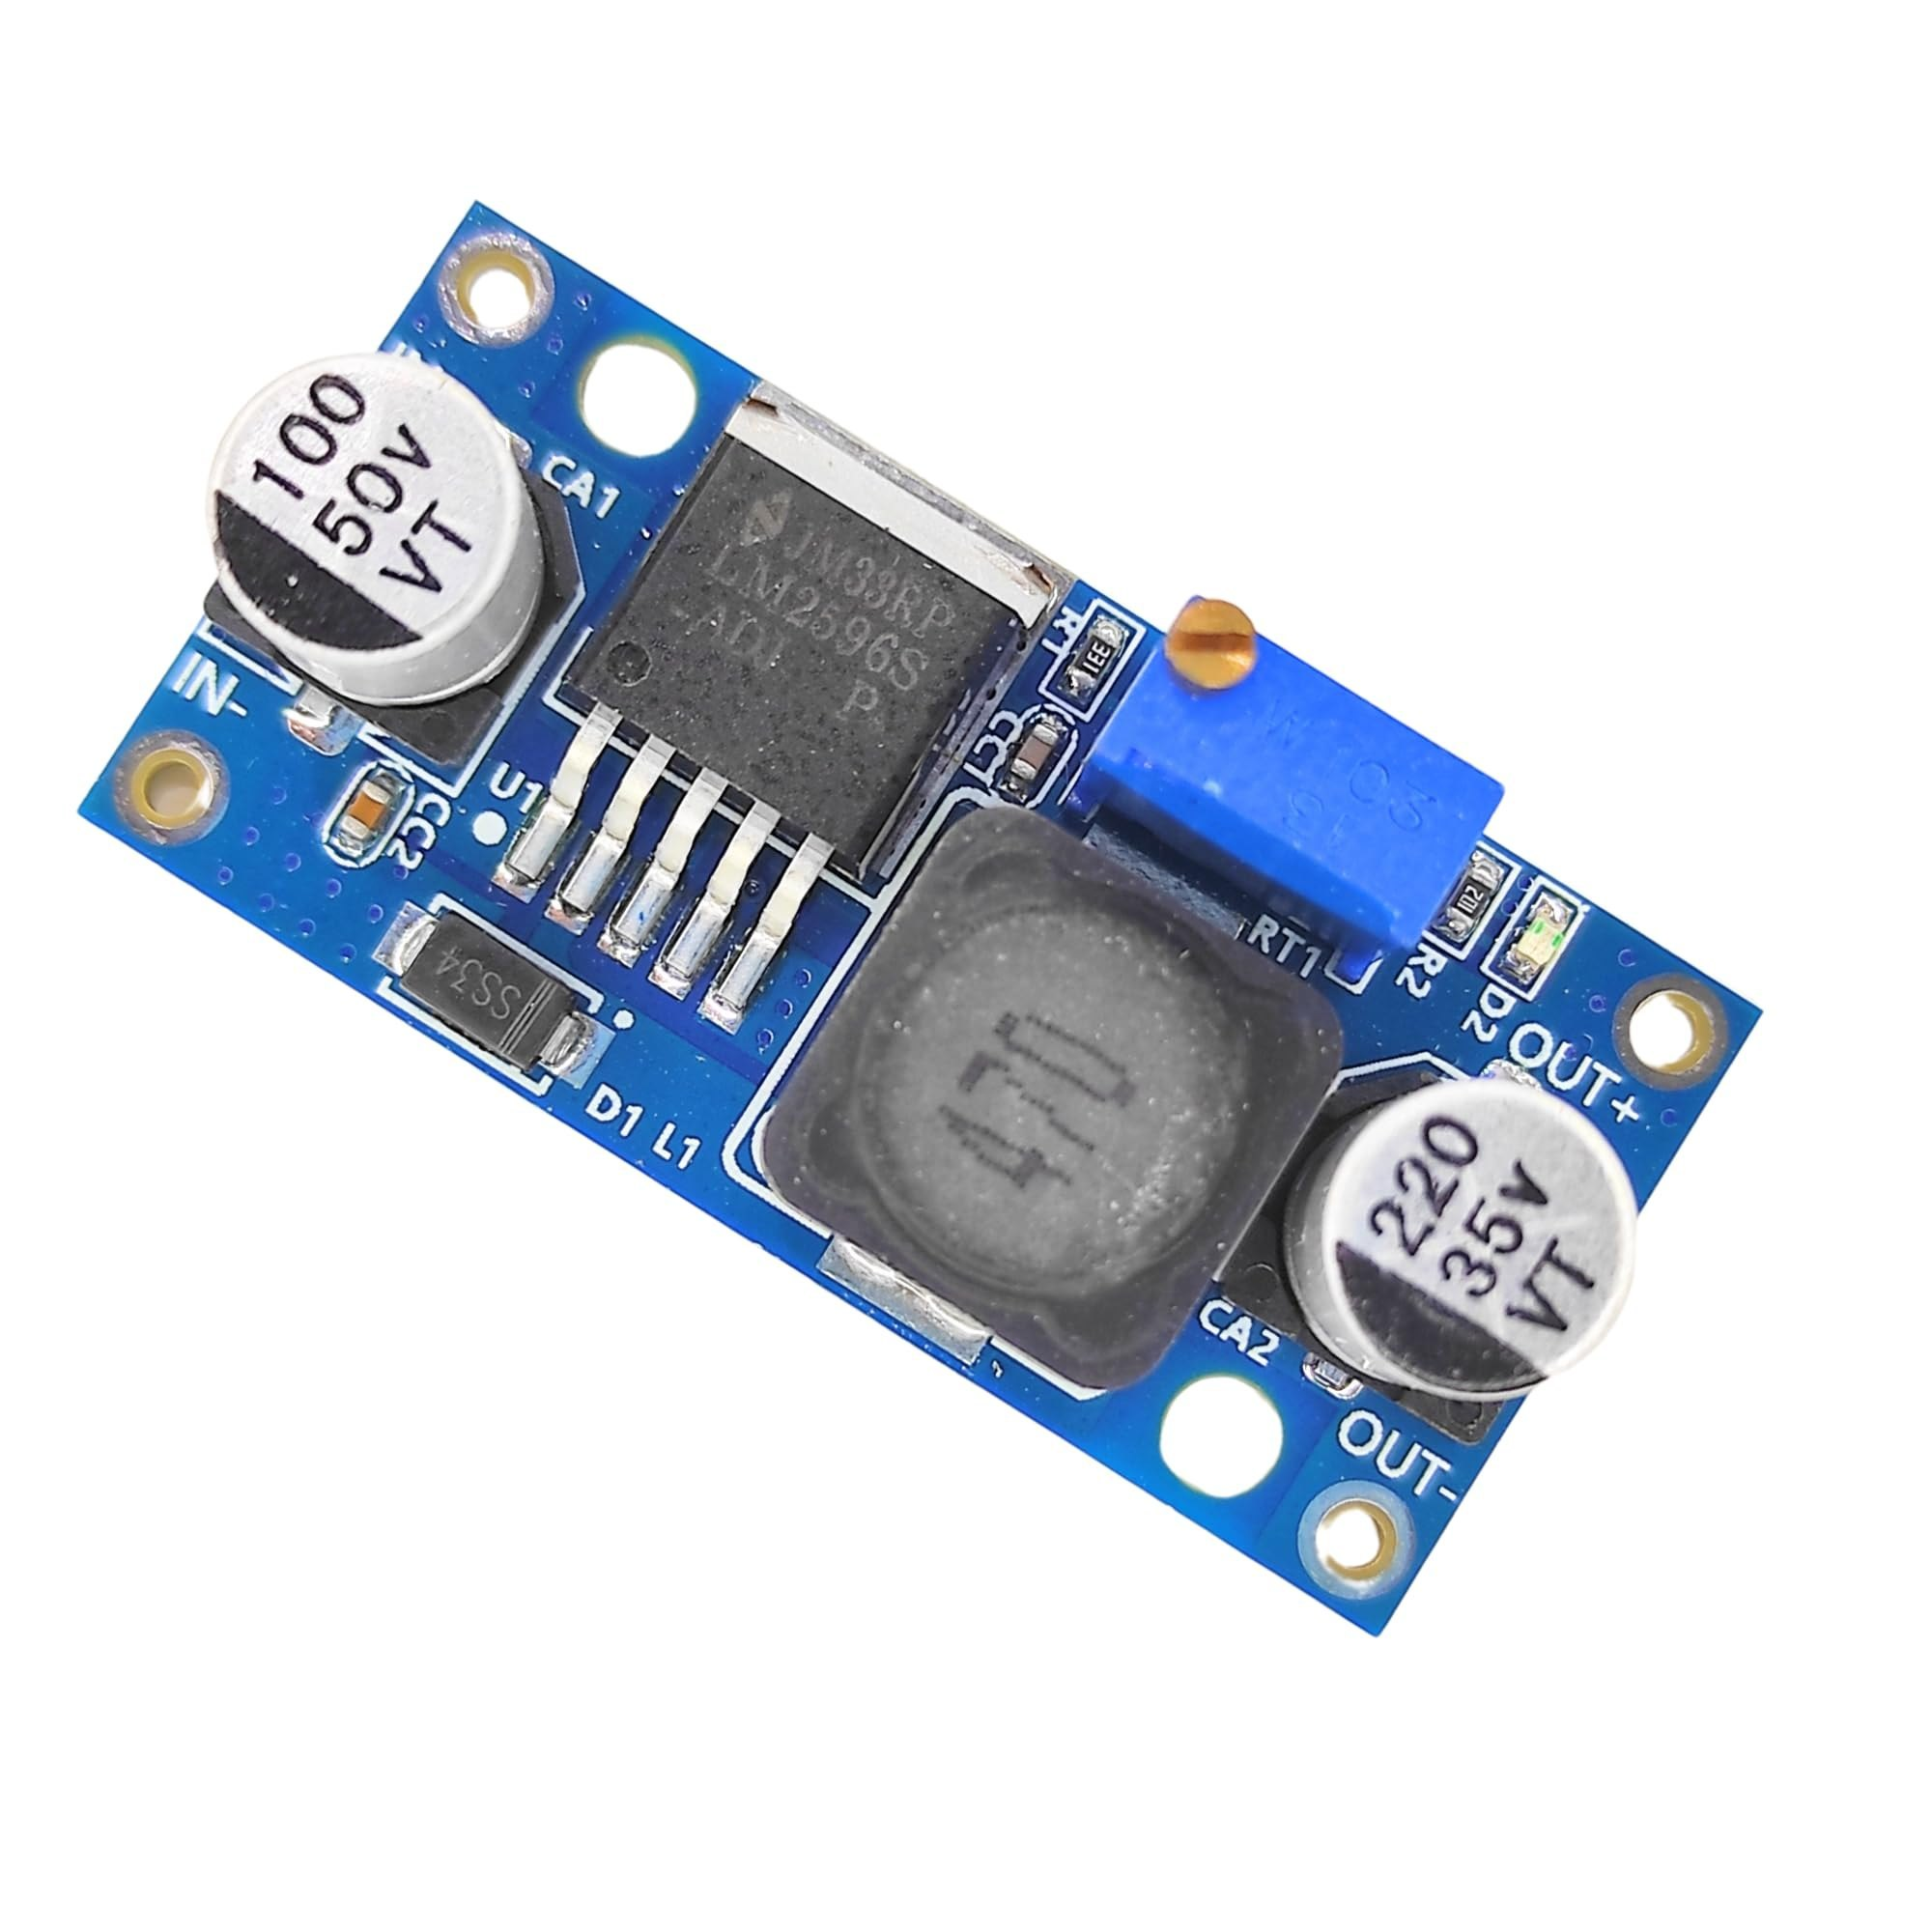
\includegraphics[width=3cm]{figures/buck_converter} &
	Regulates the 12 V input into required voltages: 6 V for the servos and 5 V for the relay and control circuits. \\
	
	NPN Transistor & 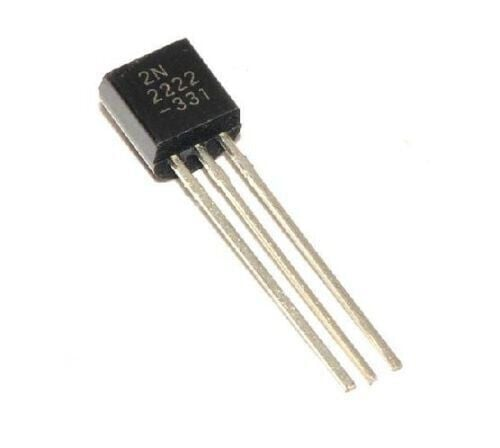
\includegraphics[width=3cm]{figures/transistor} &
	Serves as a relay driver that amplifies the Arduino’s control signal to energize the relay coil. \\
	
	Flyback Diode & 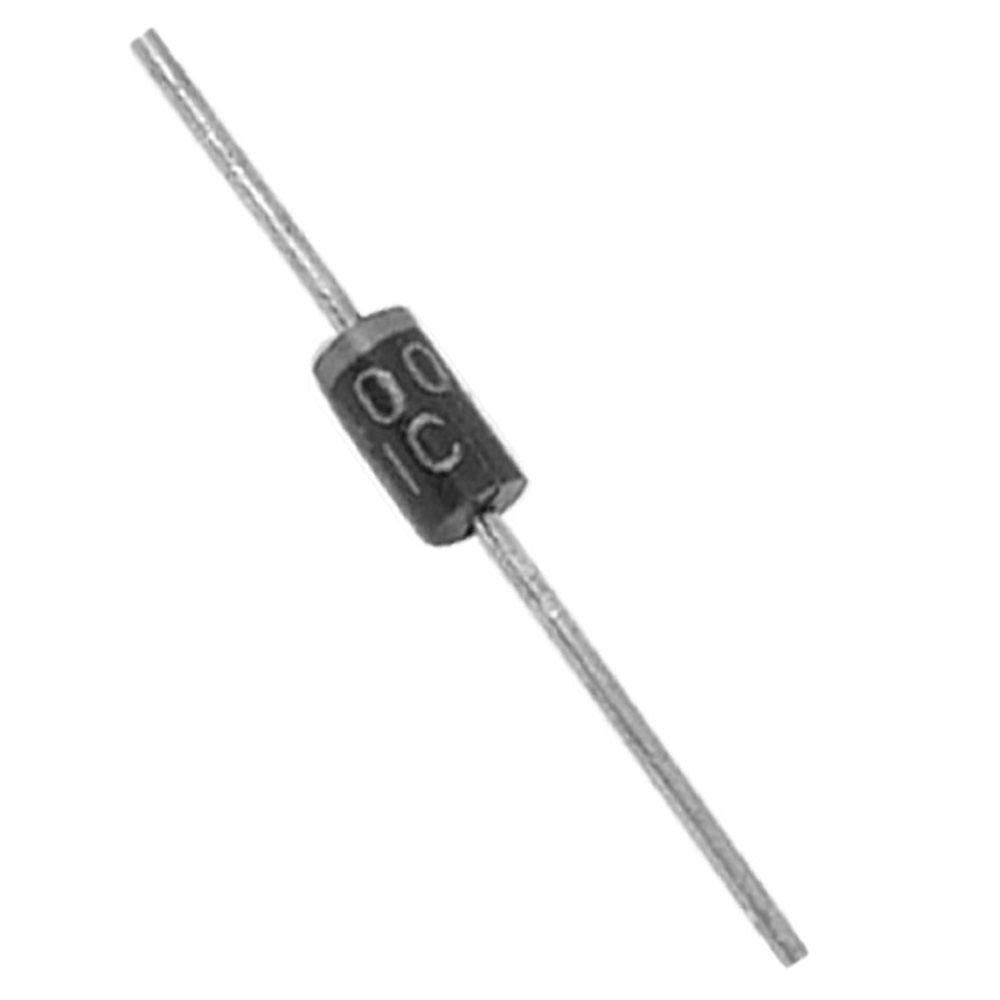
\includegraphics[width=3cm]{figures/diode} &
	Protects the transistor and other components from voltage spikes generated by inductive loads. \\
	
	Servo Motor & 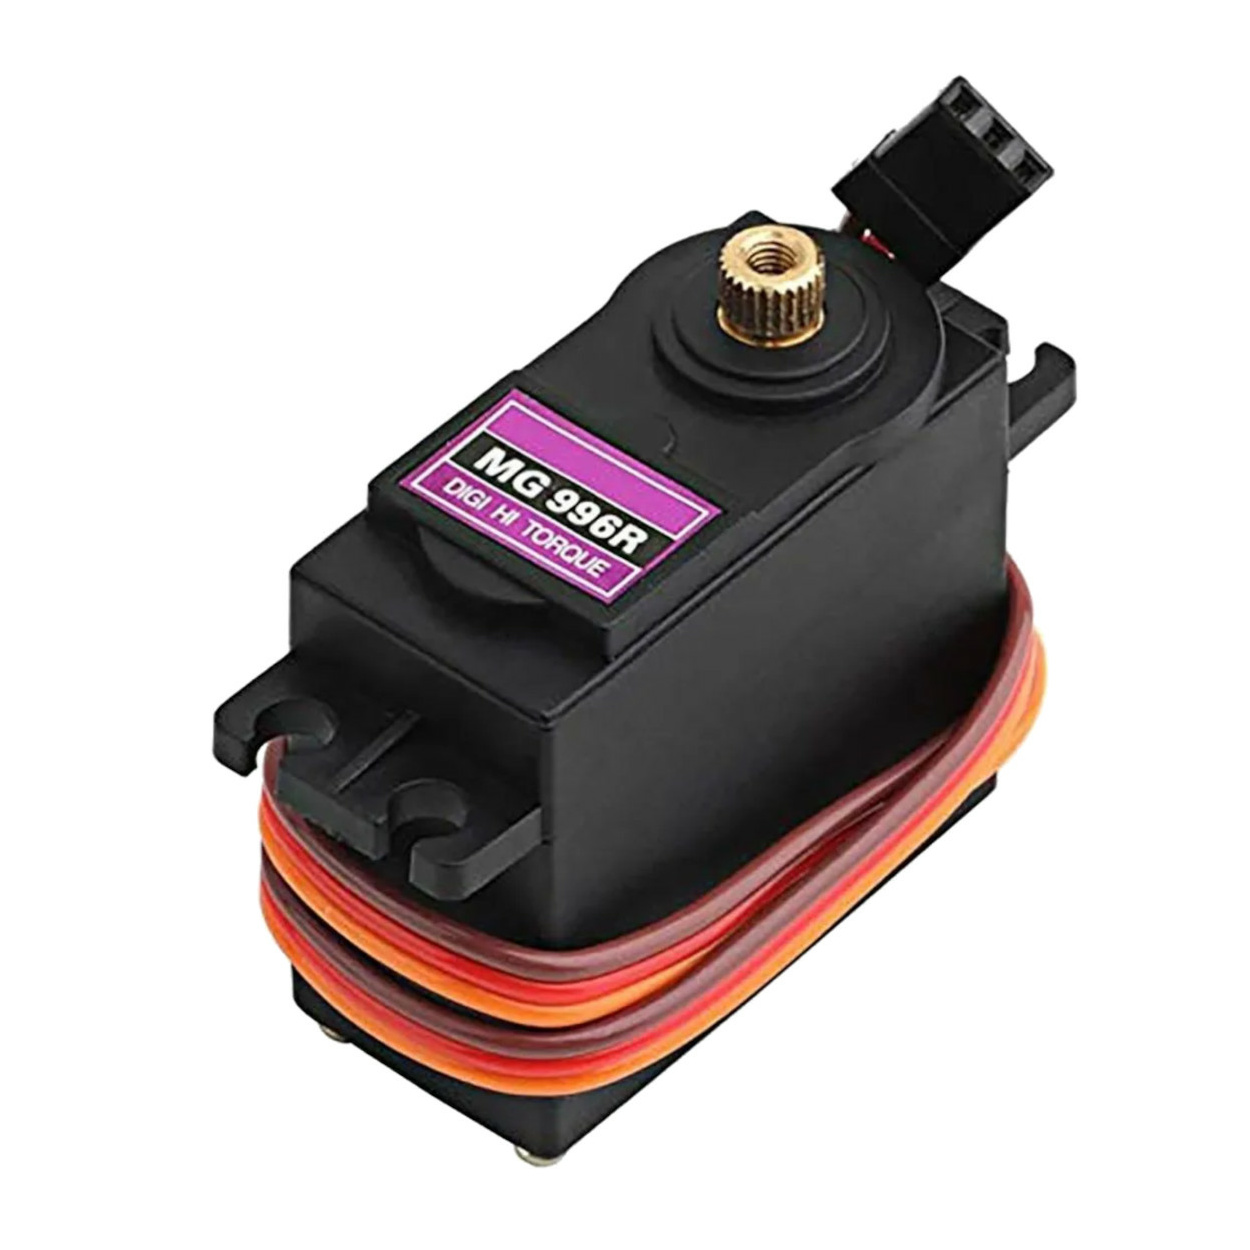
\includegraphics[width=3cm]{figures/servo_motor} &
	Controls the sorting gates that direct eggplants into Grades Extra Class, Class I, Class II, or Rejected bins after classification. \\
	
	Ball Bearings & 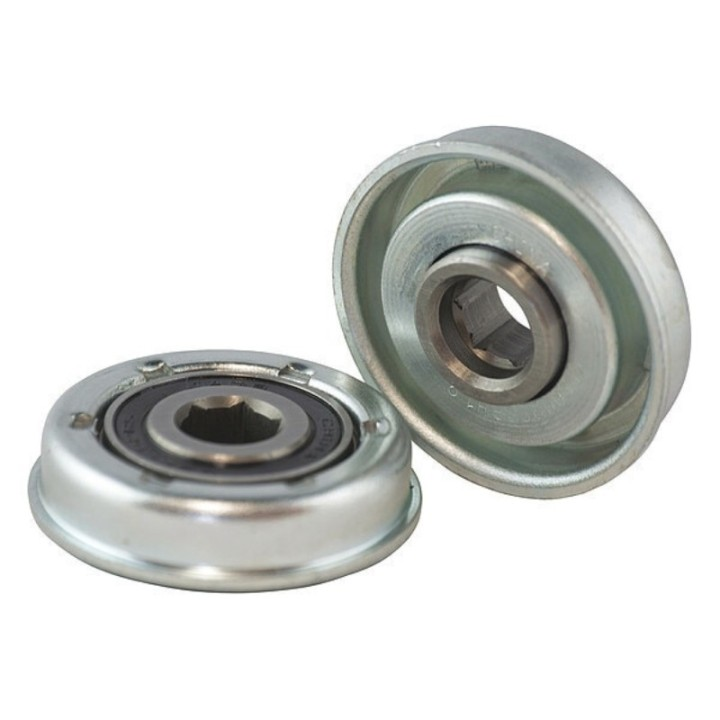
\includegraphics[width=3cm]{figures/ball_bearing} &
	This part enables the smooth rotation of the conveyors rollers by minimizing friction. It supports the conveyor belt’s movement, allowing efficient loading and consistent operation of the rollers. \\
	
	Bolts \& Nuts & 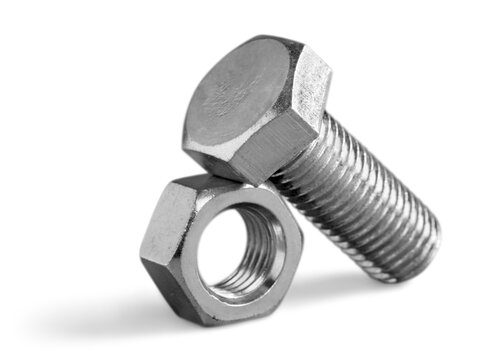
\includegraphics[width=3cm]{figures/bolts_nuts} &
	This component is used to firmly attach and hold together parts of the conveyor system, such as the motors, frame, and rollers, to keep everything stable and properly aligned. \\
	
	Wood Screws & 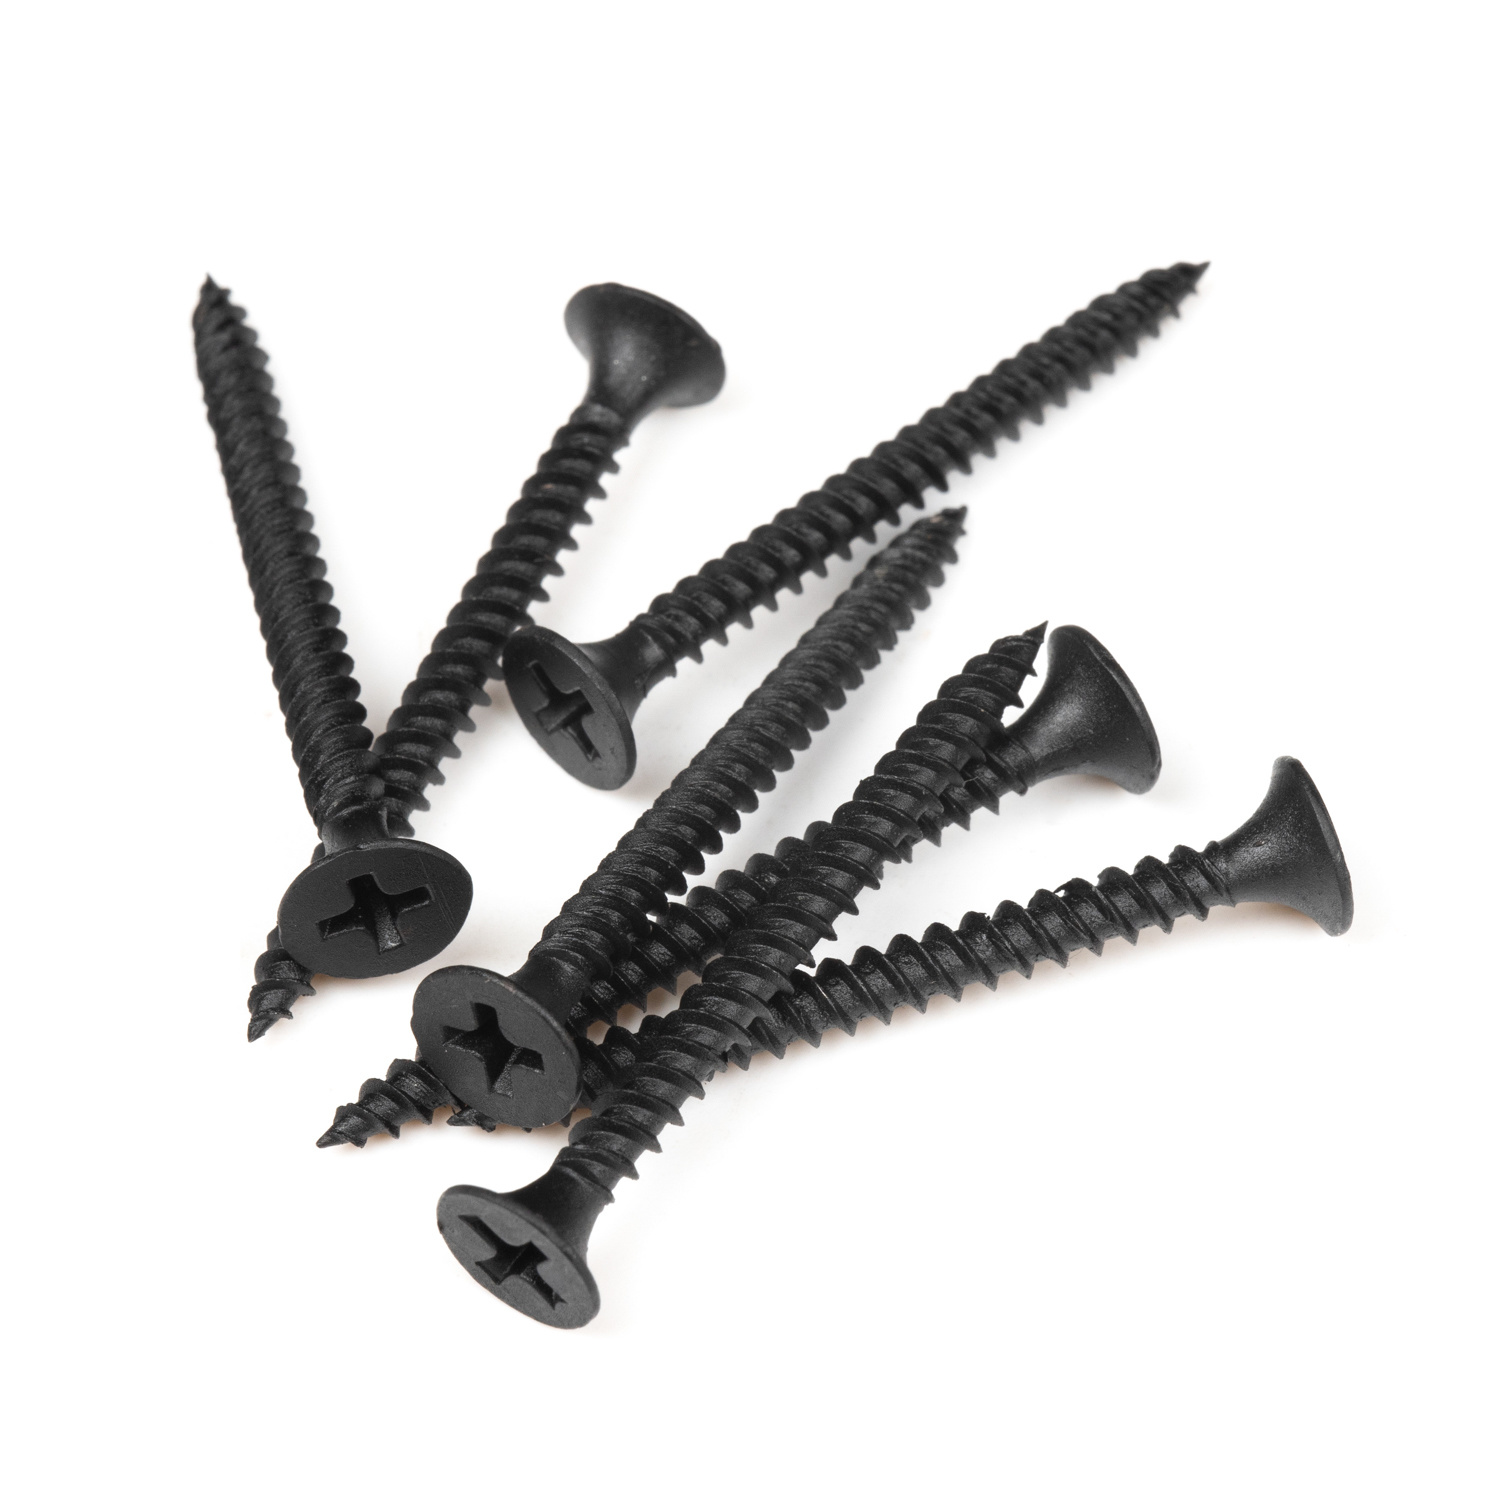
\includegraphics[width=3cm]{figures/screws} &
	This component is used to join and secure the parts of the conveyor belt system, including the wooden frame, rollers, and other sections, ensuring they are firmly attached and properly assembled. \\
	
	Conveyor Rollers &
	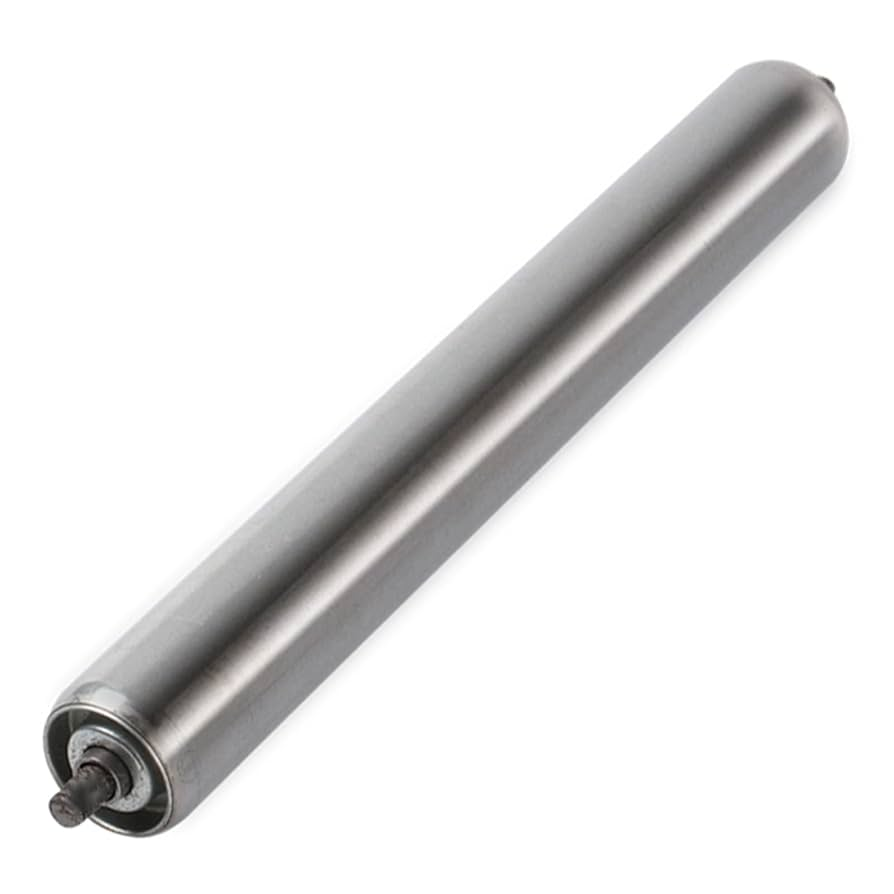
\includegraphics[width=3cm]{figures/conveyor_roller} &
	The conveyor rollers enable the smooth movement of the conveyor belt, allowing the eggplants placed on top to be transported efficiently. They also help keep the belt properly aligned to ensure stable and consistent motion during operation. \\
	
	Timing Belt Pulley &
	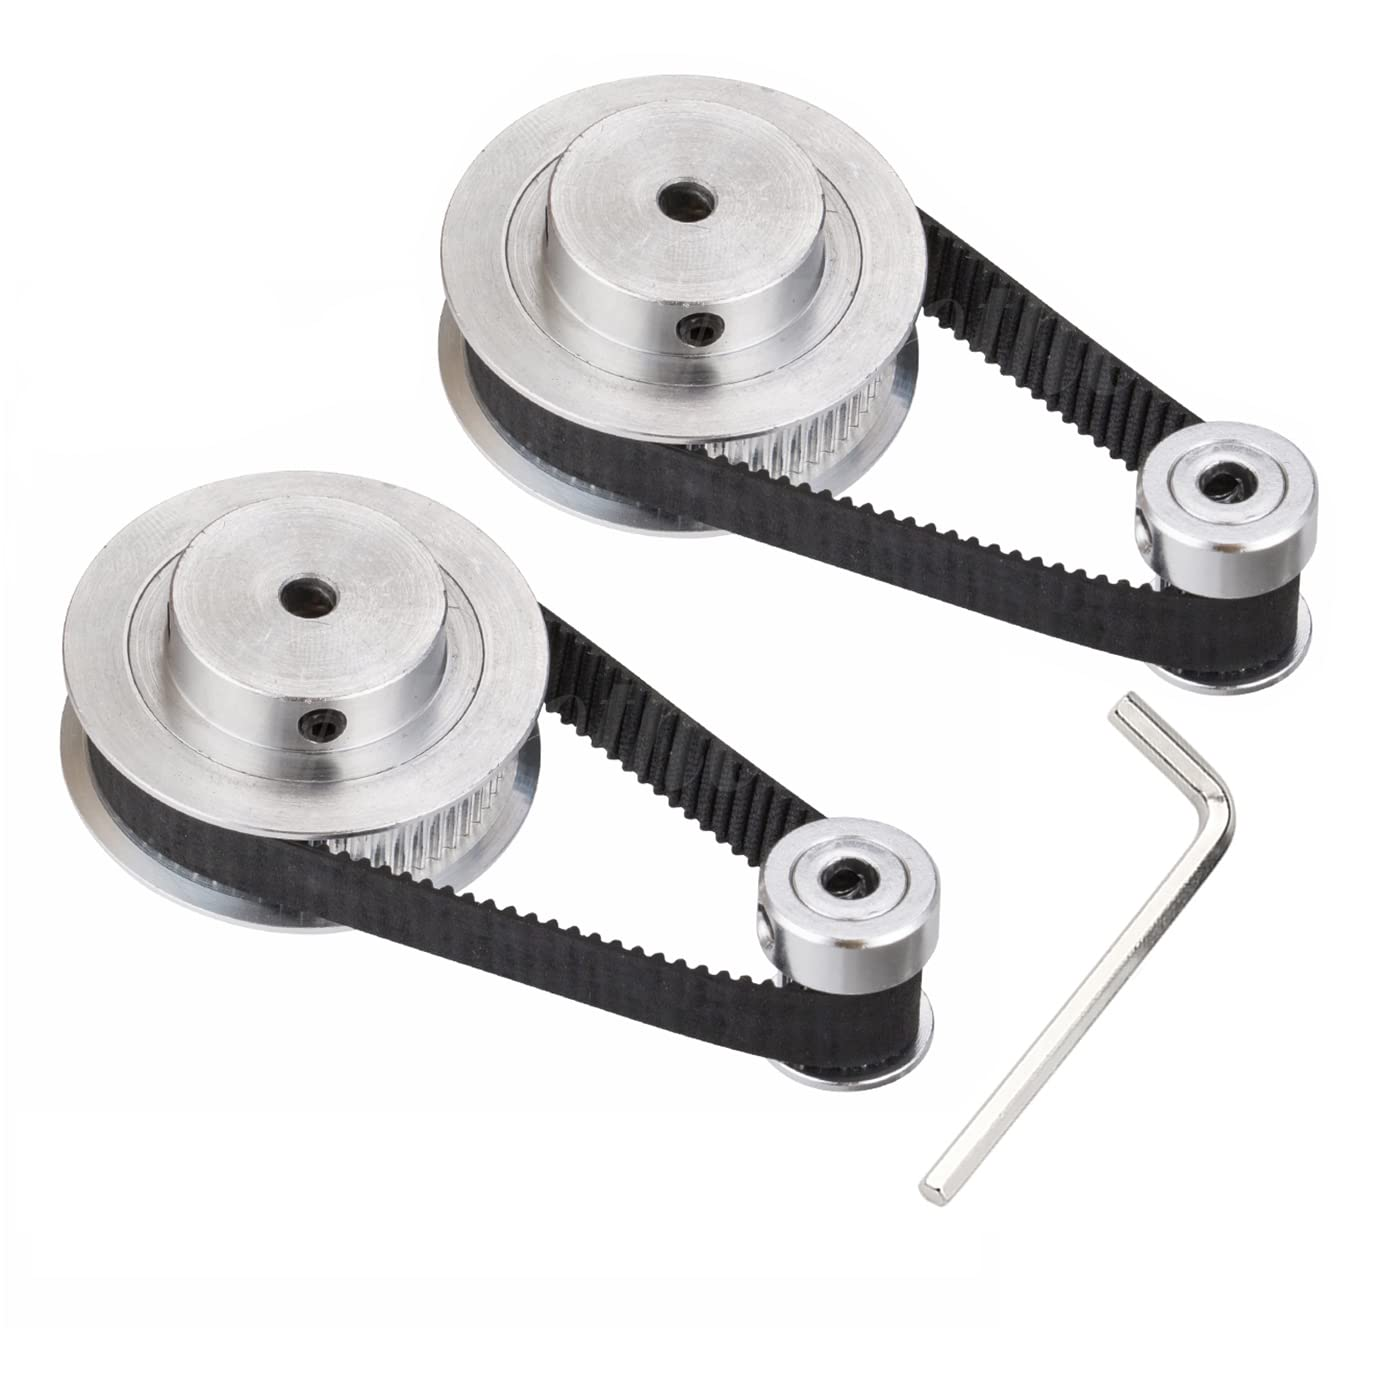
\includegraphics[width=3cm]{figures/timing_belt_pulley} &
	The timing belt pulley transfers the motor’s rotation to the rollers through a timing belt, ensuring synchronized and slip-free movement. Its toothed design keeps the rollers turning accurately and at the same time, allowing smooth and consistent movement of eggplants along the conveyor. \\
	
	Acetate Plastic &
	
\includegraphics[width=3cm]{figures/acetate} &
	The acrylic glass platform serves as a transparent base that allows the cameras positioned above and below to capture clear images of both sides of the eggplant. \\
	
	HD Webcam (Sri home SH003) &
	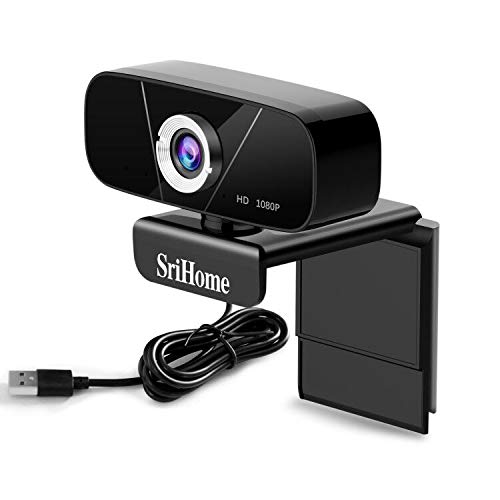
\includegraphics[width=3cm]{figures/camera} &
	This hardware component captures real-time images or video of the eggplants on the conveyor belt. The captured data is then used for image processing and analysis to identify quality and classify the eggplants accordingly. \\
	
	LED Strips &
	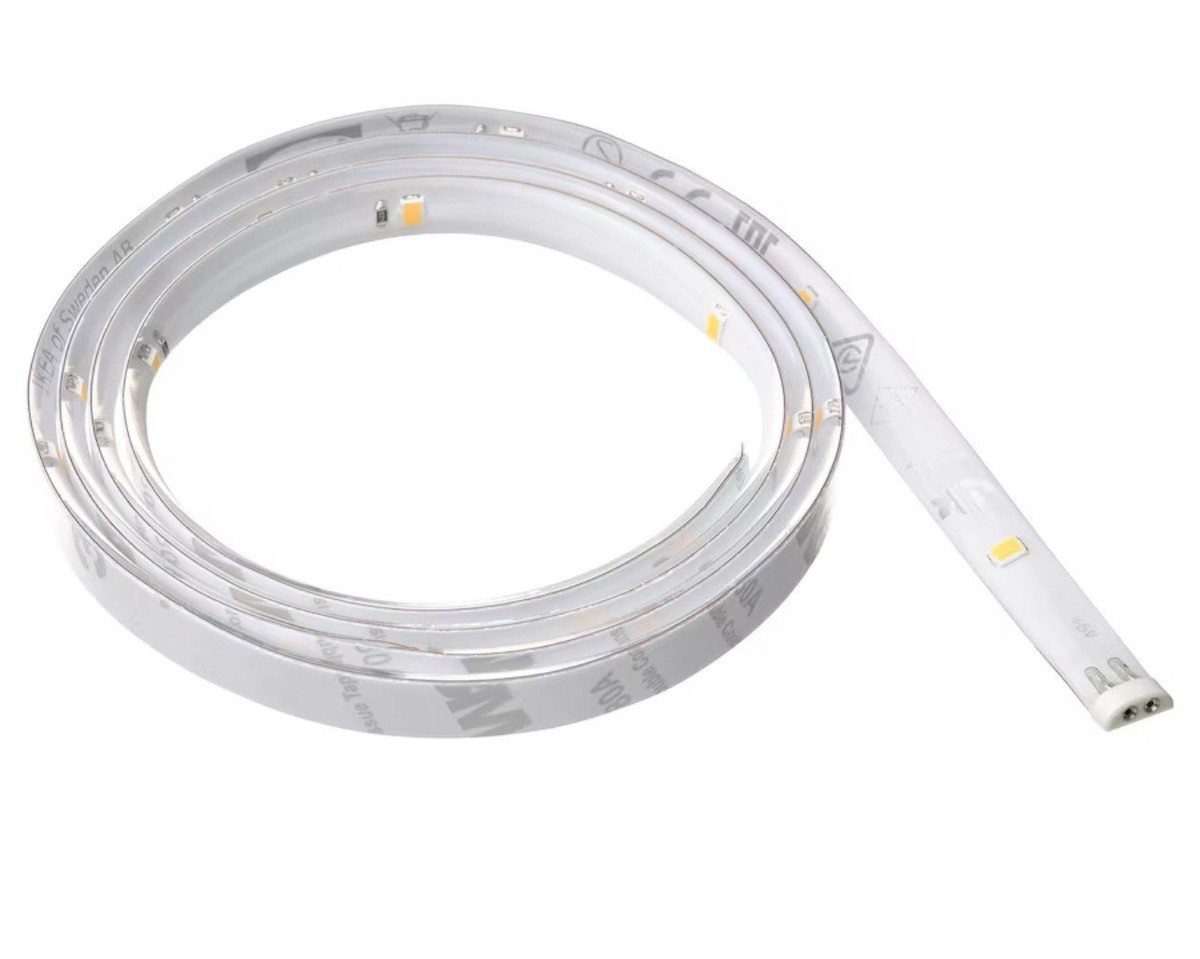
\includegraphics[width=3cm]{figures/led} &
	The LED strips give the camera the right amount of light, helping to improve the accuracy of sorting and classifying eggplants by their quality. \\
	
	Sorting Plate &
	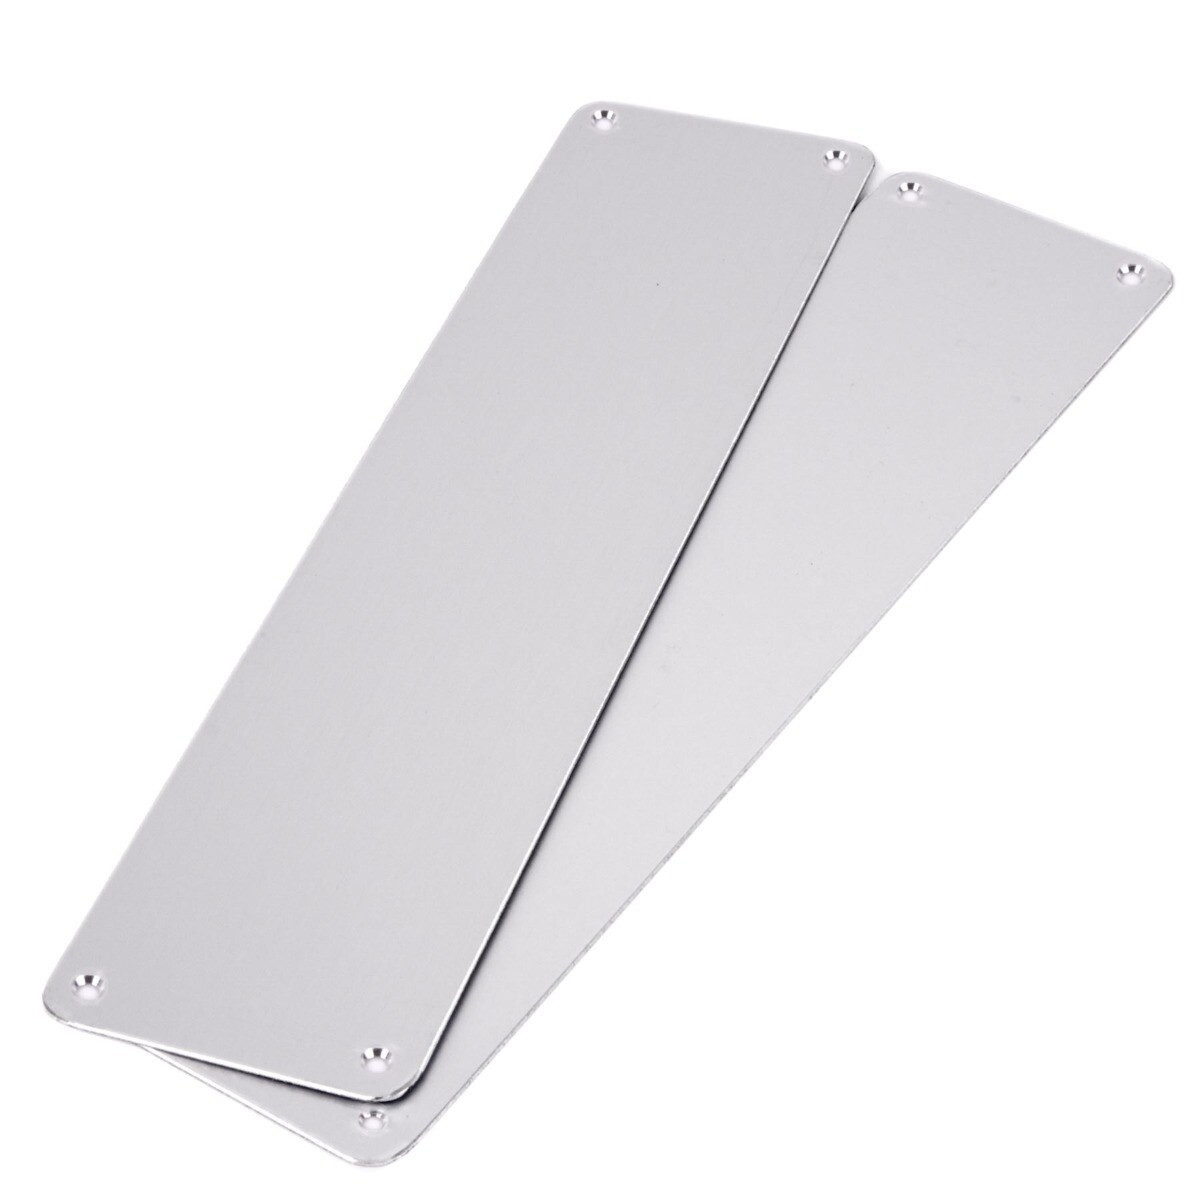
\includegraphics[width=3cm]{figures/plate} &
	Functions to redirect eggplants into their designated bins. Its smooth, durable surface minimizes friction and prevents damage during the sorting process. \\
	
	Flat Bar&
	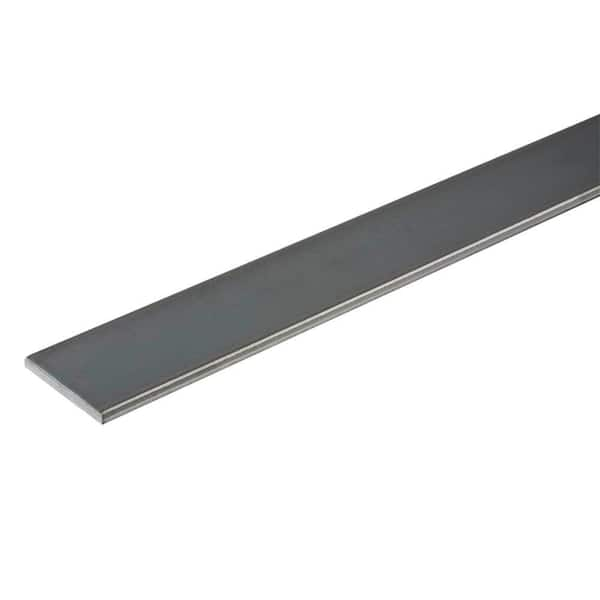
\includegraphics[width=3cm]{figures/flat_bar} &
	This part will be used as a structural foundation for the camera to mount on top of the conveyor belt. \\
	
	Wooden Planks &
	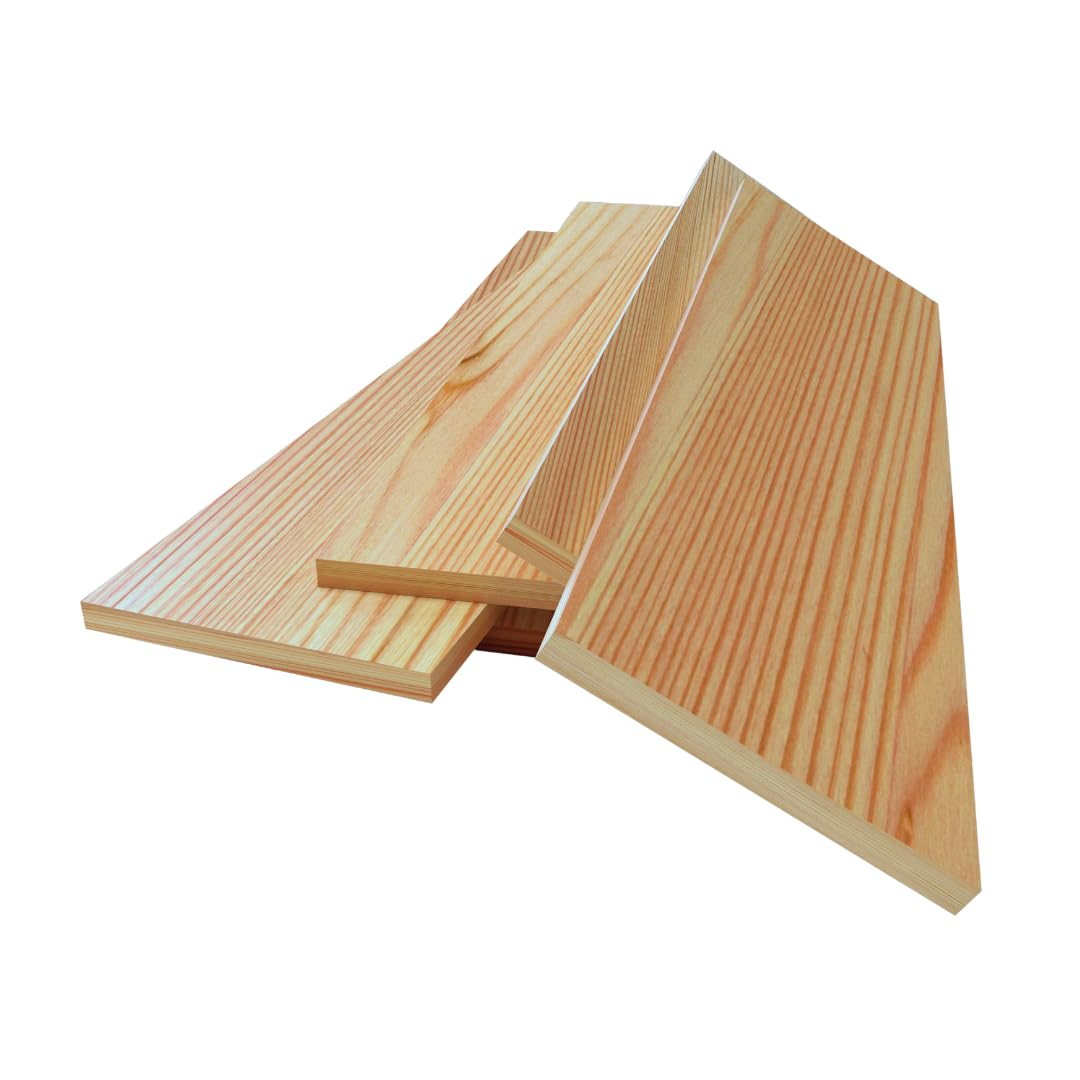
\includegraphics[width=3cm]{figures/planks} &
	Serves as the base frame that securely holds all components of the conveyor belt, ensuring the entire system remains steady during operation. \\
	
	Enclosure Box &
	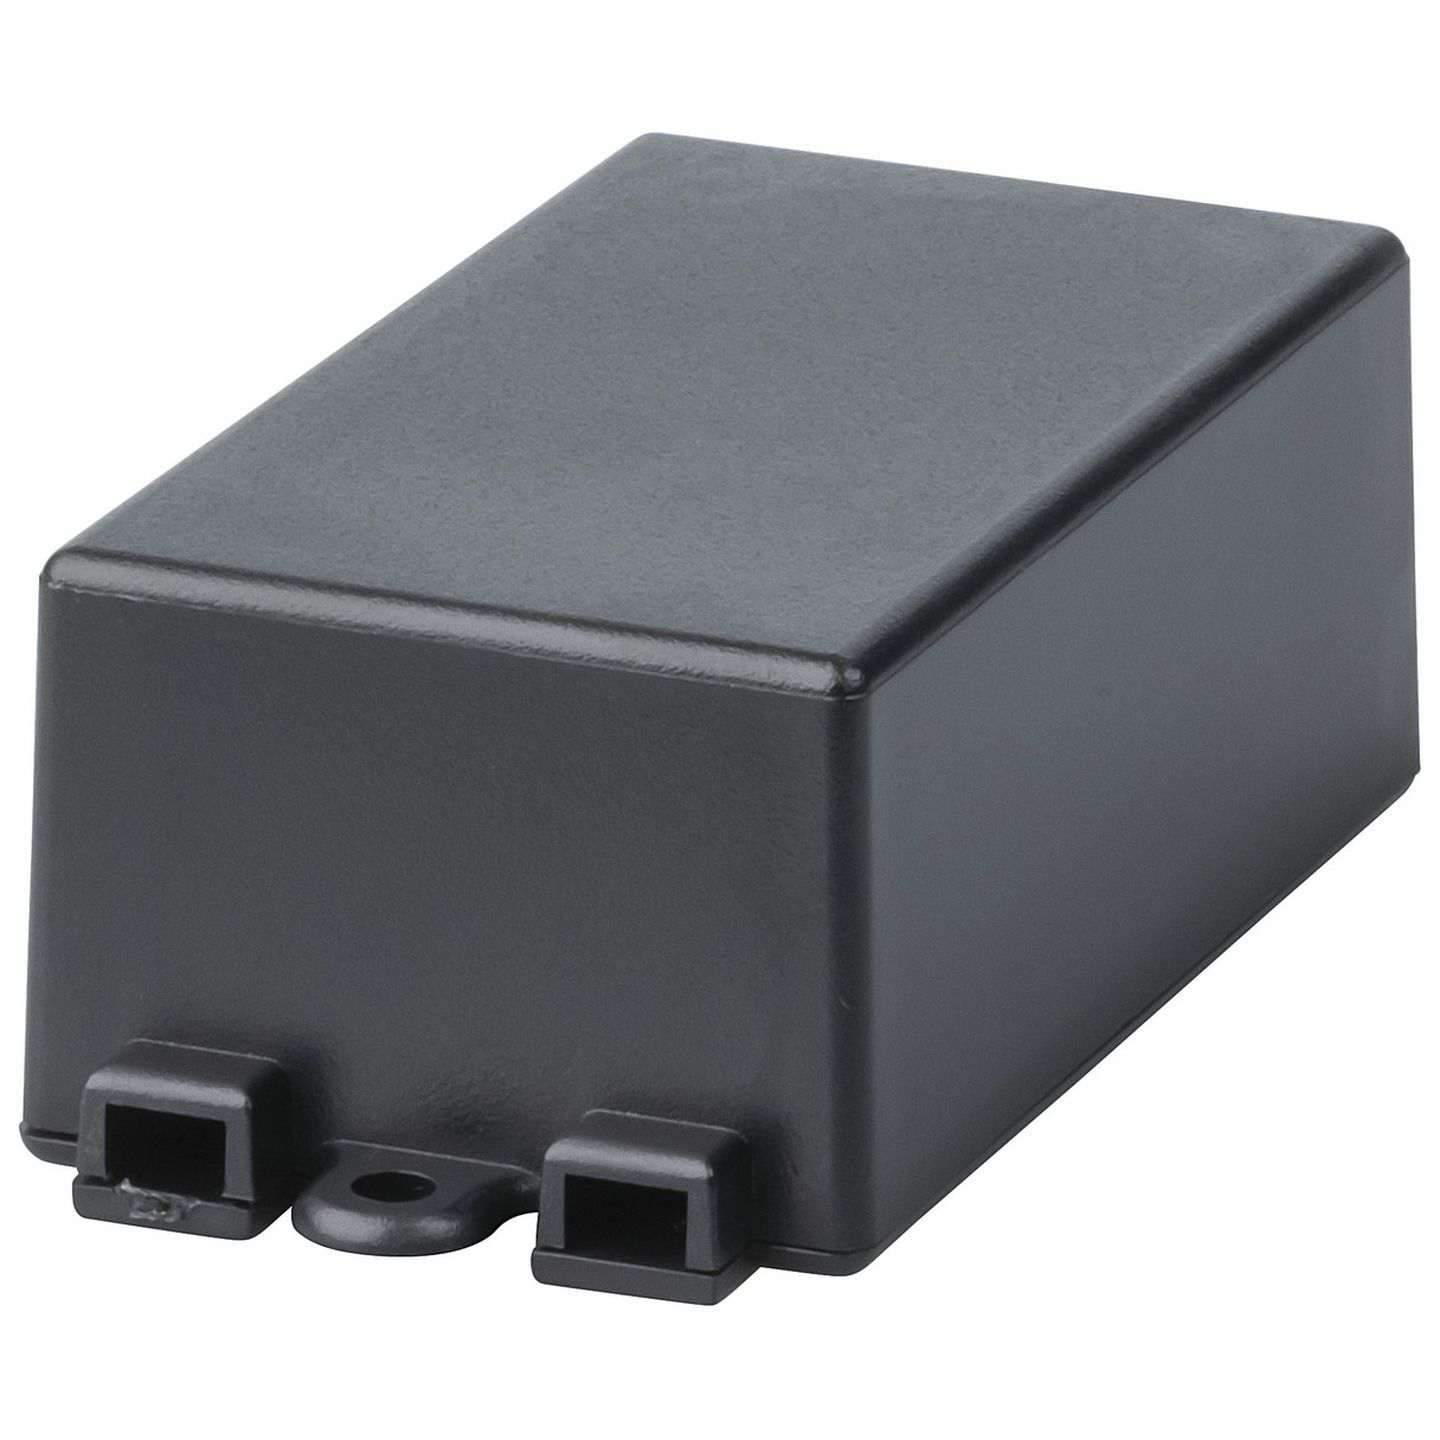
\includegraphics[width=3cm]{figures/box} &
	This will be used to keep the components (Arduino, switch, power supply, relay) arranged in one container. \\
	
	Conveyor Belt &
	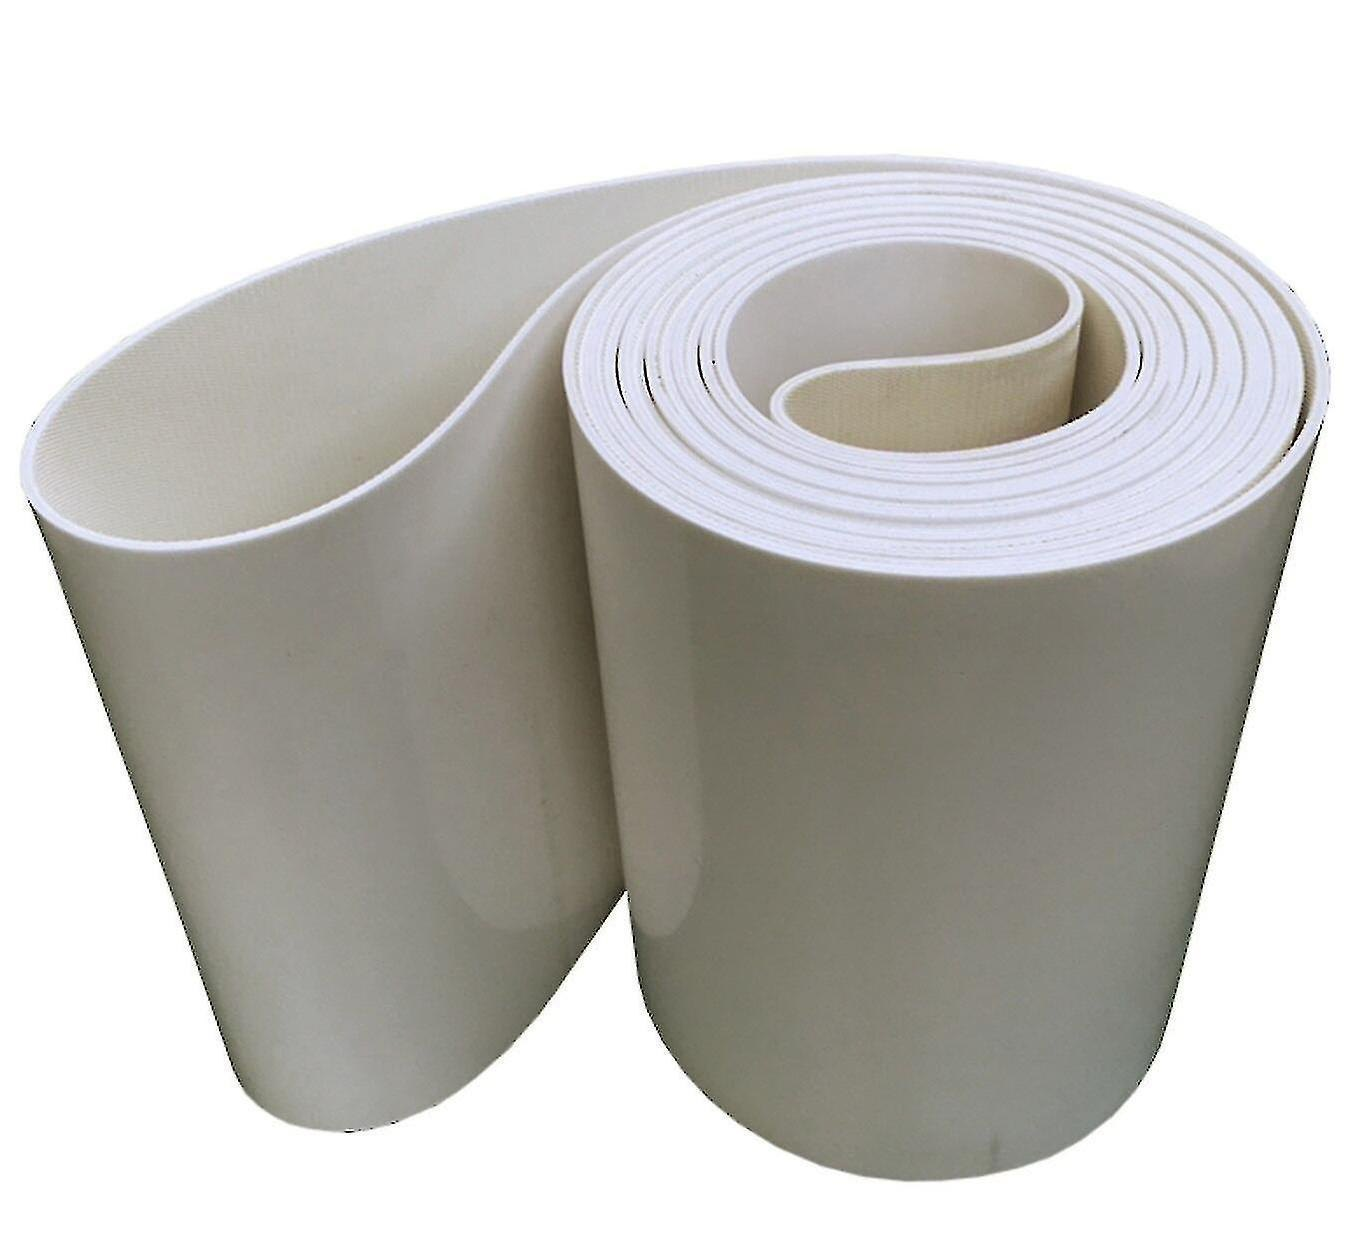
\includegraphics[width=3cm]{figures/belt} &
	Serves as the main transport surface for the eggplants, ensuring smooth and hygienic movement along the sorting path. Its non-toxic and easy-to-clean material makes it suitable for handling fresh produce while maintaining consistent motion for accurate image capture and sorting. \\
	
	Relay Module &
	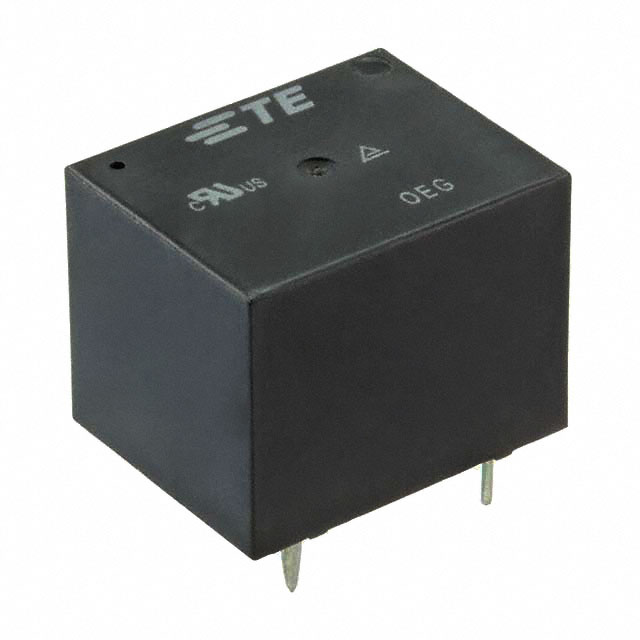
\includegraphics[width=3cm]{figures/relay} &
	Controls the DC motor by switching the 12 V supply line through a transistor-based driver circuit. \\
	
\end{longtable}

\subsection{Hardware Cost}
The estimated prices of the components required to construct the conveyor belt system are shown in Table \ref{tab:hardwarecost}. The cost, which is approximately \textpeso 8,863.00 reflects the parts needed for the construction of the conveyor belt system. The selected components ensure a balance between performance and affordability, making the system cost-effective without compromising functionality or durability using widely available materials.

\begin{longtable}{
		>{\centering\arraybackslash}m{4cm}  
		>{\centering\arraybackslash}m{4cm} 
		>{\centering\arraybackslash}m{3cm}
	}
	\caption{Hardware Cost} \label{tab:hardwarecost} \\
	\toprule
	\textbf{Components} & \textbf{Model} & \textbf{Price} \\
	\midrule
	\endfirsthead
	
	DC Motor & 775 DC Motor & \textpeso769.00 \\
	Power Supply Adapter & & \textpeso118.00 \\
	Arduino & Arduino Uno R3 & \textpeso540.00 \\
	2$\times$ & LM2596S DC-DC Step-Down & \textpeso60.00 \\
	NPN Transistor & 2N2222 & \textpeso30.00 \\
	Flyback Diode & 1N4007 & \textpeso14.00 \\
	LED Strip Lights & & \textpeso199.00 \\
	Ball Bearings & & \textpeso100.00 \\
	Bolts \& Nuts & & \textpeso200.00 \\
	5$\times$ Servo Motor & MG946R Full Metal Gear High Torque Servo & \textpeso436.00 \\
	5$\times$ Sorting Gates & UHMW-PE & \textpeso470.00 \\
	Wood Screws & & \textpeso80.00 \\
	Conveyor Rollers & & \textpeso266.00 \\
	Timing Belt Pulley & 60 teeth - 20 teeth 5mm & \textpeso200.00 \\
	Acetate Plastic & & \textpeso125.00 \\
	2$\times$ HD Webcam & SRICAM SriHome SH003 & \textpeso2,800 \\
	Flat Bar & 1'' $\times$ 1'' & \textpeso300.00\\
	Wooden Planks & & \textpeso400.00 \\
	Enclosure Box & IP65 & \textpeso150.00 \\
	Conveyor Belt & PVC Food-Grade Conveyor Belt & \textpeso1,900.00 \\
	Relay Module & SRD-05VDC-SL-C Power Relay & \textpeso45.00 \\
	\midrule
	\textbf{Total Estimated Cost:} & & \textpeso8,863.00 \\
	
	\bottomrule
	
\end{longtable}


\section{Formula}

\myequation{Some text}

\section{Tables}

\begin{center}
	\begin{longtable}{|l|l|l|}
		\caption{A sample long table.} \label{tab:long} \\
		
		\hline \multicolumn{1}{|c|}{\textbf{First column}} & \multicolumn{1}{c|}{\textbf{Second column}} & \multicolumn{1}{c|}{\textbf{Third column}} \\ \hline 
		\endfirsthead
		
		\multicolumn{3}{c}%
		{{\bfseries \tablename\ \thetable{} -- continued from previous page}} \\
		\hline \multicolumn{1}{|c|}{\textbf{First column}} & \multicolumn{1}{c|}{\textbf{Second column}} & \multicolumn{1}{c|}{\textbf{Third column}} \\ \hline 
		\endhead
		
		\hline \multicolumn{3}{|r|}{{Continued on next page}} \\ \hline
		\endfoot
		
		\hline \hline
		\endlastfoot
		
		One & abcdef ghjijklmn & 123.456778 \\
		One & abcdef ghjijklmn & 123.456778 \\
		One & abcdef ghjijklmn & 123.456778 \\
		One & abcdef ghjijklmn & 123.456778 \\
		One & abcdef ghjijklmn & 123.456778 \\
		One & abcdef ghjijklmn & 123.456778 \\
		One & abcdef ghjijklmn & 123.456778 \\
		One & abcdef ghjijklmn & 123.456778 \\
		One & abcdef ghjijklmn & 123.456778 \\
		One & abcdef ghjijklmn & 123.456778 \\
		One & abcdef ghjijklmn & 123.456778 \\
		One & abcdef ghjijklmn & 123.456778 \\
		One & abcdef ghjijklmn & 123.456778 \\
		One & abcdef ghjijklmn & 123.456778 \\
		One & abcdef ghjijklmn & 123.456778 \\
		One & abcdef ghjijklmn & 123.456778 \\
		One & abcdef ghjijklmn & 123.456778 \\
		One & abcdef ghjijklmn & 123.456778 \\
		One & abcdef ghjijklmn & 123.456778 \\
		One & abcdef ghjijklmn & 123.456778 \\
		One & abcdef ghjijklmn & 123.456778 \\
		One & abcdef ghjijklmn & 123.456778 \\
		One & abcdef ghjijklmn & 123.456778 \\
		One & abcdef ghjijklmn & 123.456778 \\
		One & abcdef ghjijklmn & 123.456778 \\
		One & abcdef ghjijklmn & 123.456778 \\
		One & abcdef ghjijklmn & 123.456778 \\
		One & abcdef ghjijklmn & 123.456778 \\
		One & abcdef ghjijklmn & 123.456778 \\
		One & abcdef ghjijklmn & 123.456778 \\
		One & abcdef ghjijklmn & 123.456778 \\
		One & abcdef ghjijklmn & 123.456778 \\
		One & abcdef ghjijklmn & 123.456778 \\
		One & abcdef ghjijklmn & 123.456778 \\
		One & abcdef ghjijklmn & 123.456778 \\
		One & abcdef ghjijklmn & 123.456778 \\
		One & abcdef ghjijklmn & 123.456778 \\
		One & abcdef ghjijklmn & 123.456778 \\
		One & abcdef ghjijklmn & 123.456778 \\
		One & abcdef ghjijklmn & 123.456778 \\
		One & abcdef ghjijklmn & 123.456778 \\
		One & abcdef ghjijklmn & 123.456778 \\
		One & abcdef ghjijklmn & 123.456778 \\
		One & abcdef ghjijklmn & 123.456778 \\
		One & abcdef ghjijklmn & 123.456778 \\
		One & abcdef ghjijklmn & 123.456778 \\
		One & abcdef ghjijklmn & 123.456778 \\
		One & abcdef ghjijklmn & 123.456778 \\
		One & abcdef ghjijklmn & 123.456778 \\
		One & abcdef ghjijklmn & 123.456778 \\
		One & abcdef ghjijklmn & 123.456778 \\
		One & abcdef ghjijklmn & 123.456778 \\
		One & abcdef ghjijklmn & 123.456778 \\
		One & abcdef ghjijklmn & 123.456778 \\
		One & abcdef ghjijklmn & 123.456778 \\
		One & abcdef ghjijklmn & 123.456778 \\
		One & abcdef ghjijklmn & 123.456778 \\
		One & abcdef ghjijklmn & 123.456778 \\
		One & abcdef ghjijklmn & 123.456778 \\
		One & abcdef ghjijklmn & 123.456778 \\
		One & abcdef ghjijklmn & 123.456778 \\
		One & abcdef ghjijklmn & 123.456778 \\
		One & abcdef ghjijklmn & 123.456778 \\
		One & abcdef ghjijklmn & 123.456778 \\
		One & abcdef ghjijklmn & 123.456778 \\
		One & abcdef ghjijklmn & 123.456778 \\
		One & abcdef ghjijklmn & 123.456778 \\
		One & abcdef ghjijklmn & 123.456778 \\
		One & abcdef ghjijklmn & 123.456778 \\
		One & abcdef ghjijklmn & 123.456778 \\
		One & abcdef ghjijklmn & 123.456778 \\
		One & abcdef ghjijklmn & 123.456778 \\
		One & abcdef ghjijklmn & 123.456778 \\
		One & abcdef ghjijklmn & 123.456778 \\
		One & abcdef ghjijklmn & 123.456778 \\
		One & abcdef ghjijklmn & 123.456778 \\
		One & abcdef ghjijklmn & 123.456778 \\
		One & abcdef ghjijklmn & 123.456778 \\
		One & abcdef ghjijklmn & 123.456778 \\
		One & abcdef ghjijklmn & 123.456778 \\
	\end{longtable}
\end{center}
\begin{table}[ht]
	\centering
	\caption{Sample Data Table}
	\label{tab:sample}
	\begin{tabular}{l c r}
		\toprule
		\textbf{Item} & \textbf{Quantity} & \textbf{Price (\$)} \\
		\midrule
		Apples & 10 & 0.50 \\
		Bananas & 5 & 0.30 \\
		Cherries & 20 & 1.20 \\
		Dates & 50 & 2.50 \\
		\bottomrule
	\end{tabular}
\end{table}
\section{Images}
\begin{figure}
	\centering
	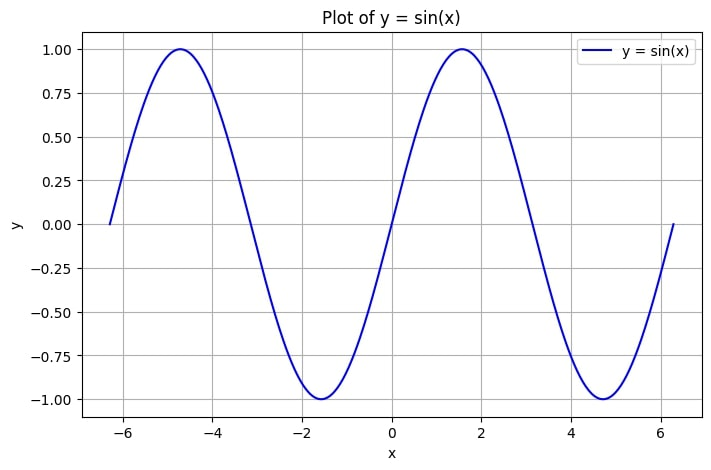
\includegraphics[width=0.7\linewidth]{figures/sinegraph}
	\caption{}
	\label{fig:sinegraph}
\end{figure}

\begin{figure}[h]
	\centering
	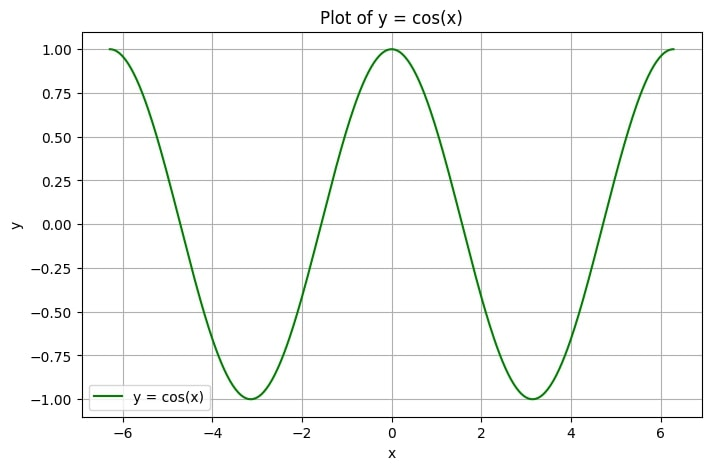
\includegraphics[height=0.3\textheight]{figures/cosinegraph}
	\caption[Cosine Graph]{Cosine Graph}
	\label{fig:cosinegraph}
\end{figure}
} 


